%%
%% Author: dariochinelli
%% 2020-09-29
%%


\section{Effetto fotoelettrico}
È uno dei possibili processi di interazione tra la radiazione elettromagnetica e la materia, come anche l'effetto Compton che vedremo più avanti. La radiazione elettromagnetica non ha solo la natura ondulatoria ma anche la natura particellare, questi effetti sono una manifestazione di questa natura particellare.

\paragraph{Esperimenti di Hertz}
Nel 1887 Hertz, studiando la scarica dei conduttori elettrizzati stimolata da una scintilla elettrica nelle vicinanze,
si accorse che tale fenomeno è più intenso se gli elettrodi vengono illuminati con luce ultravioletta.

\subsection{Esperimento di Lenard (1900)}
La \underline{scoperta} dell'effetto fotoelettrico viene attribuita a Lenard.
Scopre che il motivo dell'osservazione di Hertz è che degli elettroni vengono emessi dal catodo (elettrodo negativo) quando si fa incidere su di esso della radiazione elettromagnetica, in particolare gli esperimenti erano fatti con luce visibile e ultravioletta.
\subsection{Apparato sperimentale:} tubo di vetro sotto vuoto che contiene due elettrodi a cui viene applicata una differenza di potenziale, della luce viene fatta incidere su un elettrodo (negativo) da cui fuoriescono elettroni (fotoelettroni) attirati verso l'elettrodo positivo.
 L'emissione di elettroni viene rilevata come una corrente misurata con un amperometro.

\begin{figure}[h]
\centering
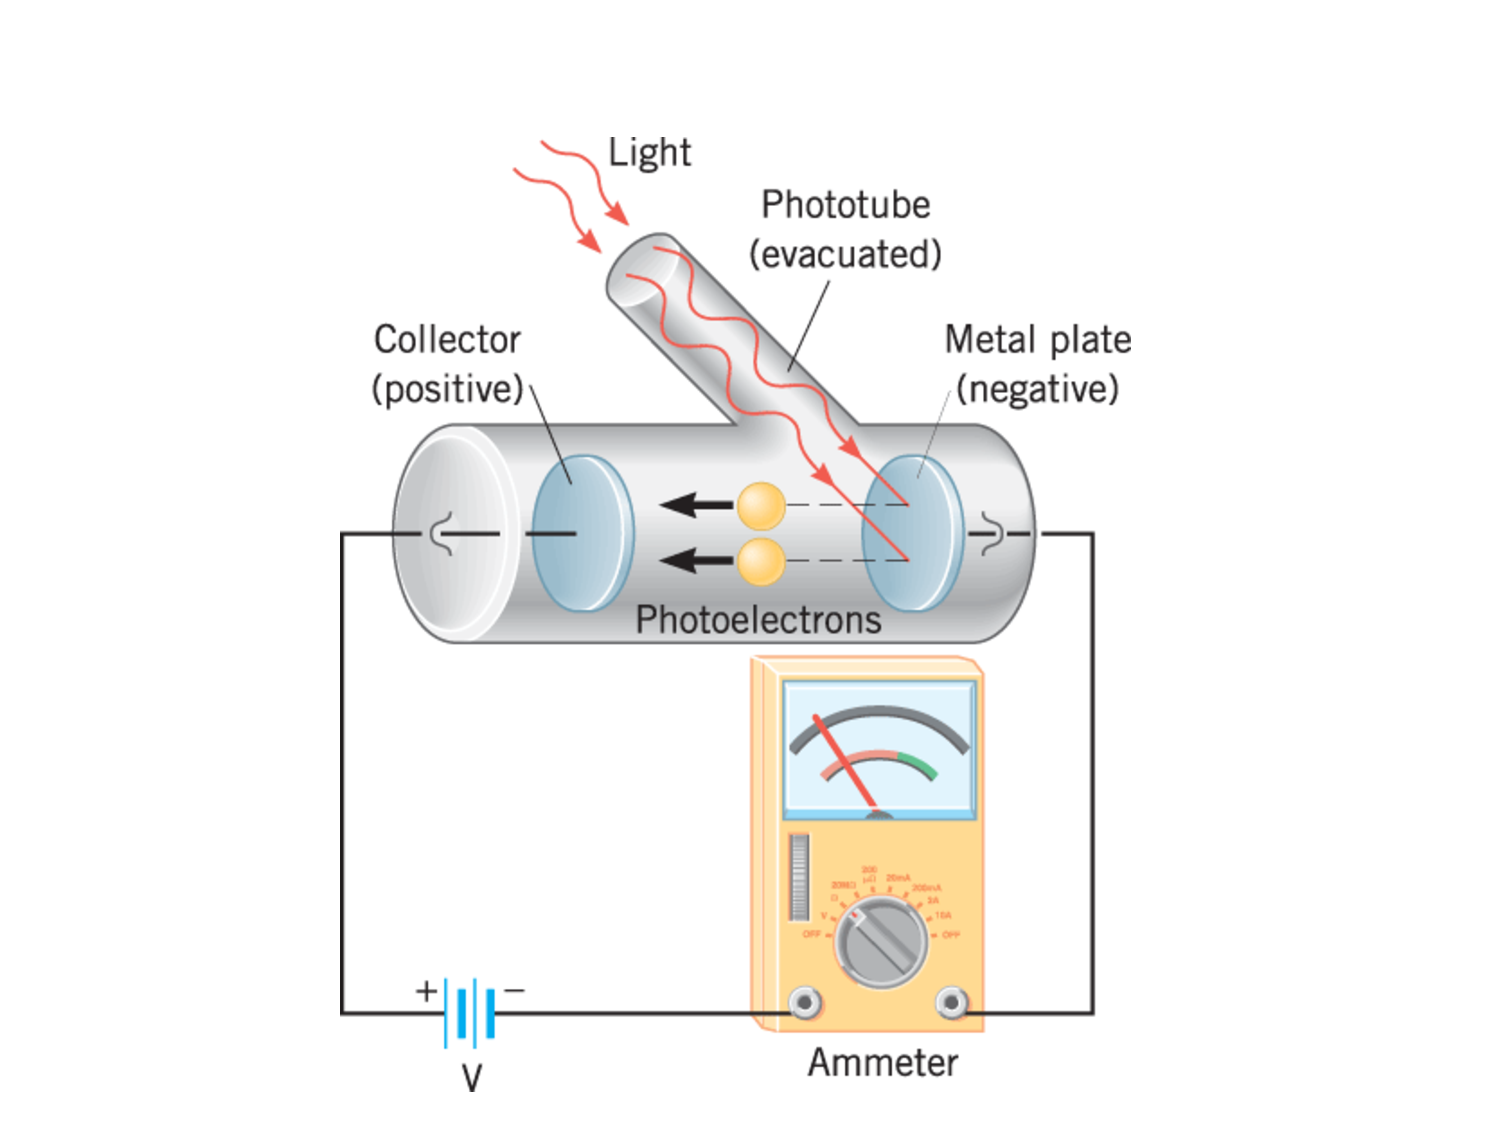
\includegraphics[scale=0.5]{/Schema_EffettoFotoelettrico}
\caption{Schema dell'esperimento di Lenard del 1900}
\end{figure}

\subsection{Risultati sperimentali}
\underline{il primo risultato sperimentale} è la corrente misurata in funzione del potenziale applicato (vedi grafico a sinistra in figura \ref{risultati_Lenard}).
Fissata l'intensità della luce incidente al valore $I_a$, quando il potenziale che applico è elevato la corrente raggiunge un livello di saturazione, riesco a raccogliere quindi tutti i fotoelettroni uscenti dal catodo.
Se porto a zero il potenziale la corrente non si annulla e nemmeno se applico un potenziale negativo. 
Significa che i fotoelettroni emessi hanno una certa energia cinetica e anche invertendo la polarità dei due elettrodi, pur venendo in parte respinti, sono ancora in grado di raggiungere il catodo.
La \textit{fotocorrente} arriva a zero quando il potenziale applicato raggiunge il valore detto \textit{potenziale di stop} $V_0$.

\begin{figure}[h]
\centering
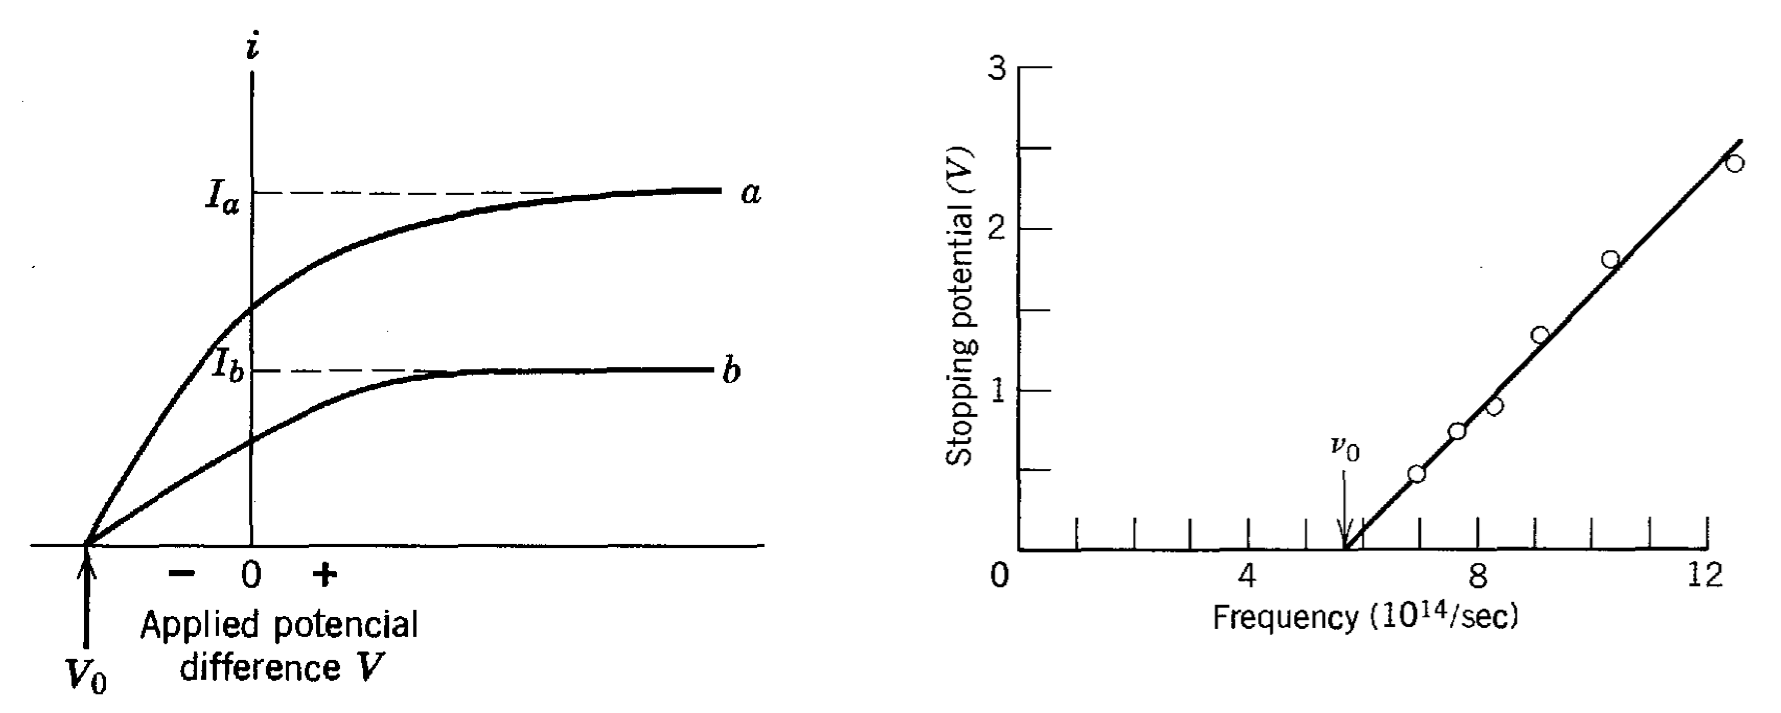
\includegraphics[scale=0.2]{/effetto_fotoelettrico}
\caption{Risultati esperimento}
\label{risultati_Lenard}
\end{figure}

L'energia cinetica massima dei fotoelettroni emessi dall'elettrodo è
\begin{equation}
K_{max} = e V_0
\end{equation}

Se considero una luce incidente con un'intensità massima $I_b$ (vedi grafico a sinistra in figura \ref{risultati_Lenard}), che si riferisce ad un'intensità minore rispetto a $I_a$, trovo un livello di saturazione minore rispetto al caso precedente ma vedo che il valore $V_0$ non cambia: l'energia cinetica massima degli elettroni non cambia, risulta essere indipendente dall'intensità della luce.

\underline{Il secondo risultato sperimentale} trovato (grazie al contributo di Millican, vedi grafico a destra in figura \ref{risultati_Lenard}) è che se grafico il potenziale di stop in funzione della frequenza della radiazione incidente trovo una relazione lineare, ma al di sotto di un certo valore di frequenza $\nu_0$ che prende il nome di \textit{frequenza di cutoff} non osservo più l'effetto fotoelettrico: ovvero non osservo più l'emissione di elettroni dall'elettrodo colpito dalla radiazione.




La fisica classica, con la teoria ondulatoria della luce, non è in grado di spiegare tre aspetti fondamentali di questo fenomeno:
\begin{enumerate}[label=\Roman{*}]
\item Poiché l'intensità della luce è proporzionale all'ampiezza del vettore campo elettrico al quadrato, il campo elettrico $\vec E$ dovrebbe aumentare all'aumentare dell'intensità della luce.
La forza applicata all'elettrone dovrebbe essere proporzionale al vettore campo elettrico e con esso l'energia cinetica degli elettroni dovrebbe aumentare, ma questo non accade: non si vede una dipendenza dell'energia cinetica dell'elettrone dall'intensità della luce incidente.

\item Esiste una frequenza di cutoff, e non si spiega il perché. Se la luce è abbastanza intensa e fornisce abbastanza energia l'effetto dovrebbe verificarsi per qualsiasi frequenza, per la teoria ondulatoria, ma non è così. 

\item Considerando una luce incidente molto debole, l'elettrone dovrebbe aver bisogno di un certo tempo per accumulare sufficiente energia per essere emesso, dovrebbe esserci un tempo misurabile in cui questo avviene.
Eppure non si misura nessun ritardo fra il momento in cui la luce incide sull'elettrodo e l'emissione dell'elettrone, l'esperimento sembra suggerire che il fenomeno avvenga istantaneamente.
\end{enumerate}

\subsection{Spiegazione dell'effetto fotoelettrico di Einstein}
La radiazione elettromagnetica è costituita da un'insieme di pacchetti di energia, che oggi chiamiamo \textit{fotoni} (denominati così da un chimico: Lewis), di energia data da
\begin{equation}
E = h \nu
\end{equation}
dove $h$ è la costante di Planck e $\nu$ è la frequenza della radiazione.

Che differenza c'è rispetto a Planck?
Planck aveva applicato la quantizzazione dell'energia agli elettroni accelerati sulle pareti di cavità, poi pensava che la radiazione si propagasse come onde di energia quantizzata, ma onde.
Einstein propone che l'energia che si irradia (scambiata tra pareti e onde nella cavità, se pensiamo al corpo nero) venga scambiata in pacchetti di quantità $h\nu$ che rimangono tali anche successivamente allo scambio.
Egli non contesta che la luce possa essere descritta in termini ondulatori, sottolinea la natura corpuscolare della radiazione in fenomeni in cui la radiazione viene emessa e assorbita.

\begin{equation}
\begin{split}
Planck \quad & \Rightarrow \quad \mbox{onde di energia quantizzata} \\
Einstein \quad & \Rightarrow \quad \mbox{pacchetti di energia quantizzata} 
\end{split}
\end{equation}

L'effetto fotoelettrico per Einstein consiste nel completo assorbimento di un fotone da parte di un elettrone del catodo, che viene appunto fotoemesso.
La spiegazione matematica è la seguente
\begin{equation}
K = h\nu - W
\end{equation}
dove l'energia cinetica dell'elettrone emesso $K$ equivale alla differenza fra l'energia del fotone $h\nu$ completamente assorbito e una quantità $W$ che è il lavoro richiesto per strappare l'elettrone dal metallo.
L'energia cinetica massima è descritta dalla legge di Einstein per l'effetto fotoelettrico
\begin{equation}
K_{max} = h\nu - W_0
\end{equation}
Dove $W_0$ prende il nome di \textit{funzione lavoro} ed è una caratteristica del metallo utilizzato e corrisponde all'energia minima dell'elettrone per uscire dal catodo.

Dalla formula di Einstein si ricava il potenziale di stop:
\begin{equation}
\begin{split}
& K_{max} = h\nu - W_0 \\
& V_0 = \frac{ h\nu}{e } - \frac{ W_0}{e }
\end{split}
\end{equation}
quindi permette di comprendere meglio la relazione lineare tra il potenziale  di stop e la frequenza, vista in figura \ref{risultati_Lenard}.
La pendenza di tale curva è $\frac{ h}{e }$ e l'intercetta all'asse delle ordinate è $\frac{ W_0}{e }$; da questo studio è anche possibile ricavare la costante di Planck, come fece Millican trovando un valore molto vicino a quello che oggi riteniamo esatto.

\newpage

Quindi Einstein ci mette nella condizione di poter rispondere ai quesiti posti in precedenza dalla fisica classica:
\begin{enumerate}[label=\Roman{*}]
\item "$K_{max}$ non dipende dall'intensità della luce" \\
Raddoppiare l'intensità della luce incidente, mantenendo la stessa frequenza, significa raddoppiare il numero di fotoni, ma il valore dell'energia di ogni fotone $h\nu$ rimane invariato e, appunto, $K_{max}$ non dipende dall'intensità della luce.

\item "Esistenza della frequenza di cutoff"\\
Se $K_{max} = 0 \quad \Rightarrow \quad h\nu_0 = W_0$ viene strappato un elettrone ma senza energia cinetica ed è quindi il limite per il verificarsi dell'effetto fotoelettrico, $\nu_0$ è la frequenza di cutoff.

\item "Non c'è un tempo di interazione"\\
L'energia è fornita in pacchetti concentrati di energia e quindi quando un fotone viene assorbito è assorbito tutto in una volta ed immediatamente si ha l'emissione di un elettrone.
\end{enumerate}

\textbf{NB:} l'effetto fotoelettrico, quindi un completo assorbimento del fotone incidente, può avvenire anche con fotoni di più alta energia del visibile (e.g. raggi X), che però andrà ad estrarre gli elettroni più legati al nucleo.

\subsection{Raffigurazione dello spettro elettromagnetico}
\begin{figure}[h]
\centering
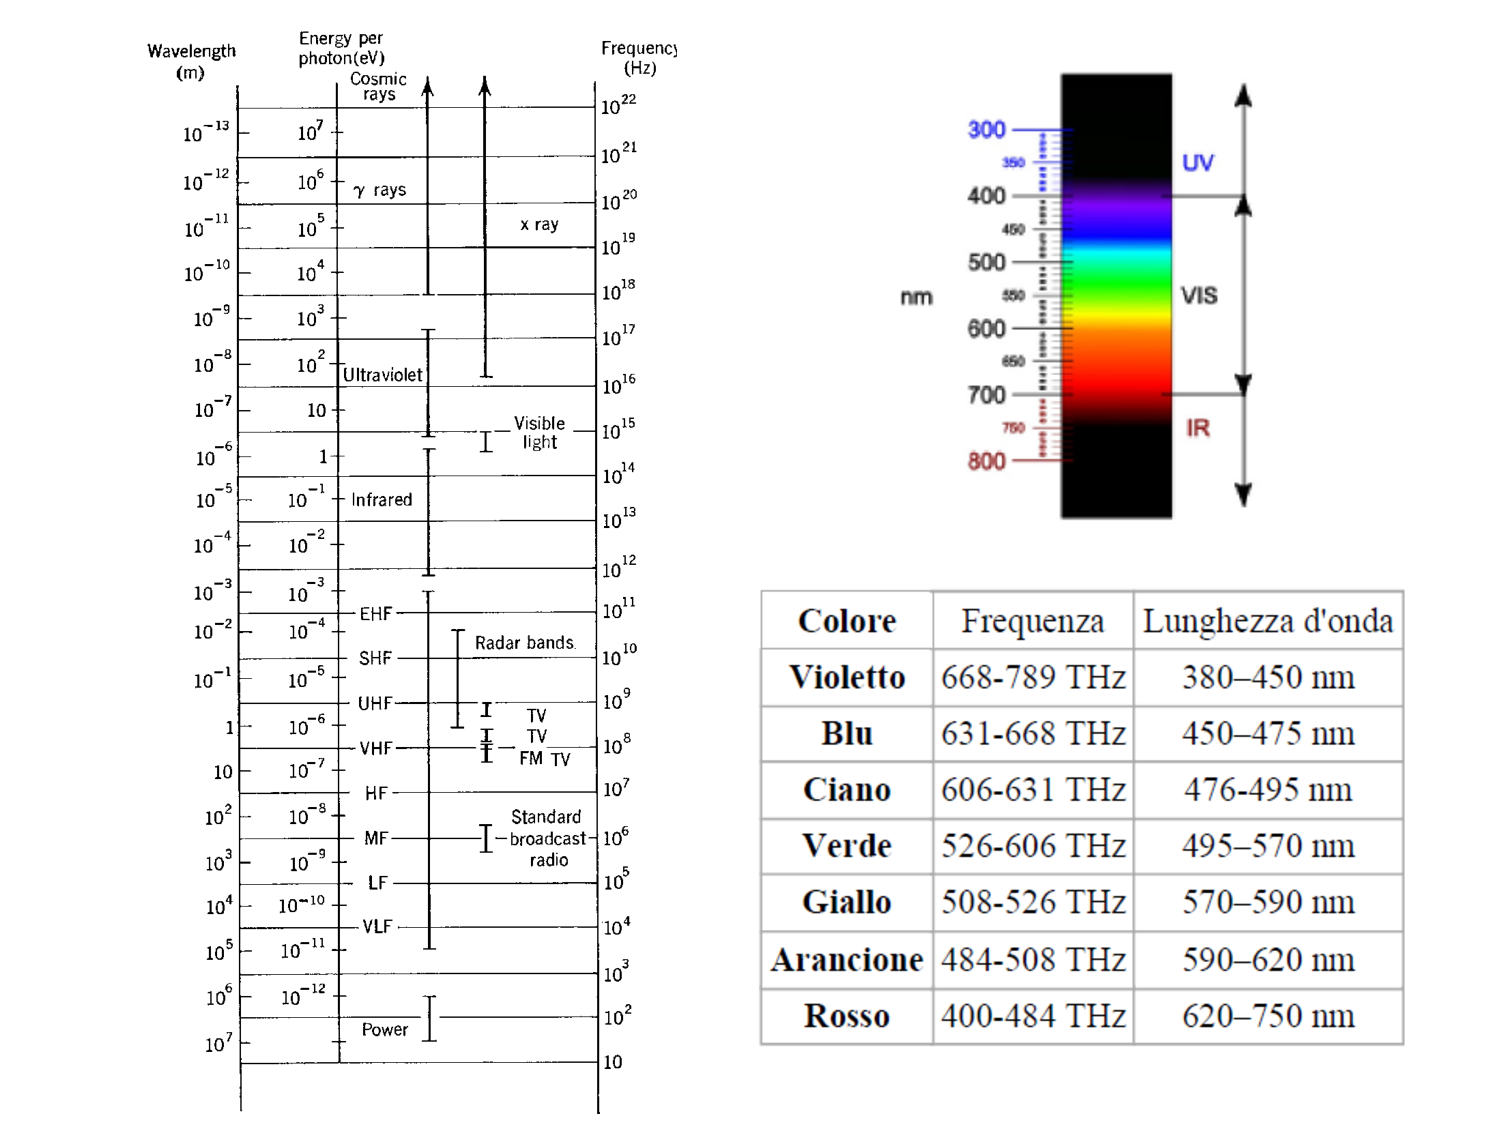
\includegraphics[scale=0.6]{/spettro_elettromagnetico}
\caption{Spettro elettromagnetico}
\end{figure}

